% In this file you should put the actual content of the blueprint.
% It will be used both by the web and the print version.
% It should *not* include the \begin{document}
%
% If you want to split the blueprint content into several files then
% the current file can be a simple sequence of \input. Otherwise It
% can start with a \section or \chapter for instance.

\chapter{Introduction}

This project is not yet complete, but intends to formalize a strengthening of the following theorem. Let $\mathbb{I} = \left[0,1\right]$ and let $n \geq 2$ be an given integer. We use $C^d$ to indicate the space of functions defined on a domain whose $d$-th derivative is continuous and use $\circ$ to indicate function composition.

\begin{theorem*}[Kolmogorov 1957]
  \label{thm:KST}
  For every $f \in C\left(\mathbb{I}^n\right) \mapsto \mathbb{R}$, there exist increasing $\psi_{p,q} \in C\left(\mathbb{I}\right) \mapsto \mathbb{R}$ that do not depend on $f$ and generally non-monotone $\chi_q \in C\left(\mathbb{R}\right) \mapsto \mathbb{R}$ that depend on $f$ and $\psi_{p,q}$, such that $f\left(x_1, x_2, \dots, x_n\right) = \sum\limits_{q = 0}^{2n} \chi_q \circ \Psi_q\left(x_1, x_2, \dots, x_n\right)$, where $\Psi_q\left(x_1, x_2, \dots, x_n\right) \equiv \sum\limits_{p = 1}^n \psi_{p,q}\left(x_p\right)$.
\end{theorem*}

\noindent This theorem is called the Kolmogorov Superposition Representation (KSR) or the Kolmogorov Superposition Theorem (KST) because Kolmogorov proved that a given multivariable ``target'' function, $f$, could be represented as a finite sum of compositions of univariate functions. 

The relevance of the KRT continues to be debated in the neural networks literature. On one side, many want to utilize the KSR to approximate unknown or expensive target functions. However, the ``inner'' functions, $\psi_{p,q}$, and ``outer'' functions, $\chi_q$, are not elementary, in the sense that they cannot be computed with a finite number of calls to basic functions. Thus, the KSR requires harmonic analysis and other side is skeptical that the it will ever be of much practical use.

Although the KST is perhaps surprising in its generality and simplicity, it has been proven in several ways, raising the question of what value is added by an additional proof? The extant proofs of the KST are of three kinds (and none have been formalized):

\begin{itemize}
    \item \textbf{Nonconstructive}: The most elegant proofs utilize the Baire Category Theorem to prove the \textit{existence} of inner and outer functions that satisfy the KST but do not suggest how to construct them.
    \item \textbf{Constructive}: Other proofs are considered to be constructive but do not even suggest a feasible algorithm to implement them in floating-point arithmetic.
    \item \textbf{Constructed}: Two constructions have been implemented in software but both utilize bad inner functions and worse outer functions, making them unworkable in floating-point arithmetic.
\end{itemize}

By ``bad" inner functions, we specifically mean they are in the Devil's Staircase family, that is, their derivative is zero almost everywhere on $\mathbb{I}$ but does not exist on a dense set of points. By ``worse" outer functions, we specifically mean that they are nowhere differentiable. Thus, even if $f$ were differentiable at some point, the chain rule does not apply to a compositions involving nowhere differentiable functions, so it cannot be used to compute a gradient under the original KSR. Most algorithms in statistics and supervised learning rely on gradients as part of some larger algorithm, so the KSR has not been useful for those purposes. 

Our goal is to construct decent inner functions and adequate outer functions that satisfy the KST and allow the chain rule to compute the gradient of $f$, which can then be implemented to floating-point arithmetic. Vitushkin proved that the inner functions in the KST cannot all be continuously differentiable. Thus, by ``decent'' inner functions, we specifically mean Lipschitz continuous functions, which satisfy $\left|\psi_{p,q}\left(x\right) - \psi_{p,q}\left(x^\prime\right)\right| \leq K\left|x - x^\prime\right|$ for some positive but finite constant $K$. The KST literature often refers to a more general definition of Lipschitz continuity (which is also termed H\"{o}lder continuity) where $\left|\psi_{p,q}\left(x\right) -   \psi_{p,q}\left(x^\prime\right)\right| \leq K\left|x - x^\prime\right|^\alpha$. Fridman and Kahane proved that the inner functions can all be weak contractions, that is, $\alpha = 1$ and $K = 1$.

Sprecher proved that there are outer functions that satisfy the KST for any target function when $\psi_{p,q}\left(x_p\right) \equiv \lambda^{p - 1} \psi\left(x_p - \frac{q}{2n}\right)$, where $\lambda > 0$ is an irrational number and $\psi$ is a weak contraction that we call the ``core'' function. However, the only known attempt to implement the Fridman-Sprecher approach in software was made by Actor, which was unsuccessful.

Actor did succeed in reparameterizing the H\"{o}lder continuous core function proposed by Sprecher, corrected by K\"{o}ppen, and proven correct by Braun and Griebel. Actor's function is parameterized via its arc length and is Lipschitz continuous by construction. While there is graphical evidence that strongly suggests Actor's function is compatible with the KST, some aspects of the approach are not fully proved, and it requires an expensive numerical inversion of Braun and Griebel's function just to achieve a few decimal places of accuracy.

Montanelli and Yang notes the importance of constructing a Lipschitz continuous KST
\begin{quote}
We have proven upper bounds for the approximation of multivariate functions $f : [0, 1]^n \mapsto \mathbb{R}$ by deep ReLU networks, for which the curse of dimensionality is lessened. The depth and the size of the networks to approximate such functions $f$ grow like $\mathcal{O}\left(\varepsilon^{-\log n}\right)$, as opposed to $\mathcal{O}\left(\varepsilon^{-n}\right)$. The proof is based on the ability of very deep ReLU networks to implement the Kolmogorov-Arnold superposition theorem.

There are many ways in which this work could be fruitfully continued. If we were able to construct a Lipschitz continuous inner function, we would be able to
obtain $\mathcal{O}\left(\varepsilon^{-1}\right)$ estimates. Actor and Knepley designed in 2017 an algorithm to compute a Lipschitz continuous inner function, but they did not provide a method to compute the outer functions.
\end{quote}
\noindent This quote reflects the fact that the outer functions depend on the inner functions, in addition to $f$. The smoother are the inner functions, the easier it is to obtain ``adequate'' outer functions that approximate a target function to a given degree of accuracy. In short, a Lipschitz continuous KST would overcome (to first order) the curse of dimensionality when approximating a target function on $\mathbb{I}^n$. 

Also, target functions in statistics, such as log-likelihood functions, typically depend on $N$ data points and the cost of evaluating them directly is polynomial (at best) in $N$. Once the outer functions have been calibrated to the target function, the KSR of the target function can be evaluated in parallel in essentially constant wall time regardless of $n$ or $N$. These savings could be enormous in computationally intensive applications, such as Markov Chain Monte Carlo or Large Language Models.

There are several open questions that are not even investigated in the KST literature:
\begin{enumerate}
    \item Can some proper subset of the inner functions be continuously differentiable (or smoother)? We show that if $0 < q < 2n$, then $\psi_{p,q} \equiv \lambda^{p - 1} \psi\left(x_p - \frac{q}{2n}\right)$ is continuously differentiable.
    \item Does the core function depend on $n$, apart from being evaluated at $x - \frac{q}{2n}$? We show that $\psi$ is universal, although $\lambda$ depends on $n$ in a simple fashion.    
    \item Can the set of points where $\psi$ is not differentiable be finite? We show that $\psi$ is not differentiable if $x = 1$ and $q = 0$ or if $x = 0$ and $q = 2n$ but is differentiable on $\left(-1,1\right)$.
    \item Can $\psi$ be approximated to floating-point precision? We show that $\psi$ can be quickly approximated to any degree of accuracy. 
\end{enumerate}

Our approach is unique in that we first construct a function with the requisite properties and then show that it is a viable core function in the KSR. Chapter \ref{ch:CoreFunction} uses basic real analysis --- most of which is already formalized in the Mathlib library used by the Lean software --- to show that our candidate for $\psi$ is increasing, Lipschitz continuous, and not continuously differentiable. In addition, since $\psi$ can be represented as a series, it is essential to demonstrate that the series converges uniformly, which is an improvement over the other constructions in the KST literature whose functions only converge pointwise. As a result, $\psi$ can be evaluated to double precision in fewer than a hundred floating point operations, and its derivative can be evaluated at double that cost (albeit to less accuracy).

Chapter \ref{ch:Injectivity} establishes in Lean that $\Psi_q\left(x_1, x_2, \dots, x_n\right) \equiv \sum\limits_{p = 1}^n \lambda^{p -1} \psi\left(x_p - \frac{q}{2n}\right)$ is injective for each $q$ when $\lambda$ is an algebraic number or a transcendental number. The proof is only slightly different from the one Sprecher has relied upon for decades that essentially extended the rational number field with an irrational $\lambda$. We instead extend a subfield of constructible numbers with a nonconstructible $\lambda$. Constructible numbers have fallen out of fashion but can, in principle, be constructed with a compass and straightedge.

Chapter \ref{ch:OuterFunctions} is the least complete but is devoted to the outer functions in the KSR. Kahane utilized the notion of a Helson set, which is a subset with the characterizing property that every continuous function over this subset can be represented as a convergent Fourier series. Kahane proved (albeit in French) necessary and sufficient conditions for a subset of $\mathbb{I}^{2n + 1}$ to be a Helson set, which essentially requires applying some function to each $\Psi_q$ that is not a polynomial of degree $n - 1$ or lower. Although Lean has an extensive and very general implementation of core concepts in topology, it does not currently include anything on Helson sets, so several obscure lemmas will need to be proved in Lean to allow our KST proof to go through.

\chapter{Core Function}\label{ch:CoreFunction}

\section{Main Definitions}\label{sec:MainDefinitions}

The atomic element of our KSR is the first-kind Chebyshev polynomial. Let $j$ be a generic integer that is usually non-negative, but is used in various ways in different contexts here.
\begin{definition}[Chebyshev polynomial of the first kind]
  \label{def:T}
  \leanok
  Let $r$ be a real number. The first-kind Chebyshev polynomial in $r$ with index $j$ is defined recursively as
  \begin{align*}
T_j\left(r\right) \equiv 
\begin{cases}
1 & \text{if } j = 0 \\
r & \text{if } j = 1 \\
2 r T_{j - 1}\left(r\right) - T_{j - 2}\left(r\right) & \text{if } j > 1
\end{cases}
  \end{align*}
\end{definition}
\noindent The Mathlib library used by Lean (version 4) actually has a more general definition of $T_j$ in its Chebyshev module that allows the index to be a negative integer and the argument to be a complex number, although that level of generality is unnecessary here. Mathlib also provides a metatheorem that can be used to tersely prove many properties of Chebyshev polynomials via induction on $j$. For example, see this extensive \href{https://fungrim.org/topic/Chebyshev_polynomials/}{list} of proven (albeit not by Lean) properties of Chebyshev polynomials.

We use $T_j$ with $j = 2^m$ to define partial sums that approach our candidate for a core function.
\begin{definition}[$k$-th order approximator]
  \label{def:approx}
  \uses{def:T}
  \lean{ψₖ}
  \leanok
  $\psi_k\left(r\right) \equiv \threesevenths + \offset + \halfsum{0}{k}{r}$, where $k \in \mathbb{N}$
\end{definition}
\begin{definition}[Core function]
  \label{def:core}
  \uses{def:T}
  \lean{ψ}
  \leanok
  $\psi\left(r\right) \equiv \threesevenths + \halfsum{0}{\infty}{r}$.
\end{definition}
\noindent For an overview of expanding a function in terms of Chebyshev polynomials, see Trefethen.

\section{Repeatedly Used Lemmas}\label{sec:RepeatedlyUsedLemmas}

When $j = 2^m$, Chebyshev polynomials follow a specialized recursion that drives subsequent lemmas.
\begin{lemma}[Doubling]
  \label{lem:TT_recursion}
  \uses{def:T}
  \lean{TT_recursion}
  \leanok
  $\TT{m + 1}{r} = 2\TT{m}{r}^2 - 1$, where $m$ is a natural number.
\end{lemma}
  
\begin{proof}
  \leanok
  Since $2^{m + 1} = 2 \times 2^m$, we can write $\TT{m + 1}{r} = T_{2 \times 2^m}\left(r\right)$. It is already proven by induction in Mathlib (TODO: add succinct explanation) that a Chebyshev polynomial whose index is a product can be written as a composition of two Chebyshev polynomials, so $T_{2 \times 2^m}\left(r\right) = T_2 \circ \TT{m}{r}$. It follows from Definition \ref{def:T} that $T_2\left(r\right) = 2r^2 - 1$, so $T_2 \circ \TT{m}{r} = 2\TT{m}{r}^2 - 1 = \TT{m + 1}{r}$.
\end{proof}

\begin{lemma}[Fixed points]
  \label{lem:fixed_points}
  \lean{fixed_points}
  \uses{lem:TT_recursion}
  \leanok
  The only two fixed points of the mapping $2 \TT{m}{r}^2 - 1 \mapsto \TT{m + 1}{r}$ are $-\frac{1}{2}$ and $1$ (but both are repellent).
\end{lemma}

\begin{proof}
  \leanok
  The mapping from Lemma \ref{lem:TT_recursion} implies a quadratic equation, $2y^2 - y - 1 = 2\left(y + \frac{1}{2}\right)\left(y - 1\right) = 0$ for the fixed points whose only two solutions are $y^\ast = -\frac{1}{2}$ and $y^\ast = 1$. The derivative of the mapping at a fixed point is $4y^\ast$, which is greater in magnitude than $1$, so both fixed points are repellent. (TODO: The repellent part is not formalized but not critical)
\end{proof}
\noindent If either fixed point is reached, the remaining terms in $\psi$ become a convergent geometric series.
\begin{lemma}[Partial geometric series]
  \label{lem:geometric}
  Let $b > 1$ be a real number. $\sum\limits_{m = j}^k b^{-m} = \frac{b^{1 - j} - b^{-k}}{b - 1}$.
\end{lemma}
\begin{proof}
  Mathlib has theorems on geometric series (TODO: add succinct explanation).
\end{proof}

\section{Uniform Convergence}\label{sec:UniformConvergence}

Let $\mathbb{T} = \left[-1,1\right]$ and $t \in T$. The infinite sum in the definition of $\psi$ converges uniformly to \emph{some} function on $\mathbb{T}$, although it is \underline{not yet known} whether it can be written in terms of special functions. 

\begin{lemma}[]
  \label{lem:summable}
  \uses{def:core}
  \lean{ψ_summable}
  \leanok
  $\psi$ is summable over $\mathbb{T}$.
\end{lemma}
  
\begin{proof}
  \uses{lem:TT_recursion, lem:geometric}
  \leanok
  We utilize the Weierstrass M-test. Since $\TT{0}{t} = t \in \mathbb{T}$, Lemma \ref{lem:TT_recursion} with induction on $m$ implies that $\TT{m}{t} = 2\TT{m - 1}{r}^2 - 1 \in \mathbb{T}$. Since $\left|8^{-m} \TT{m}{t}\right| \leq 8^{-m}$ and $\sum\limits_{m = 0}^\infty 8^{-m} = \frac{8}{7}$ by Lemma \ref{lem:geometric} with $b = 8$, $\psi$ is a well-defined function on $\mathbb{T}$.
\end{proof}
\noindent However, Lemma \ref{lem:summable} would not hold for $\left|r\right| > 1$.
\begin{lemma}[]
  \label{lem:not_summable}
If $\left|r\right| > 1$, then $\psi\left(r\right)$ is not summable, so $\psi$ is undefined outside of $\mathbb{T}$.
\end{lemma}

\begin{proof}
It suffices to show that $\lim\limits_{m \uparrow \infty} 8^{-m} \TT{m}{r} \neq 0$. If $m = 0$, then $\TT{0}{r} = r$ is a polynomial of degree $1$ with a leading coefficient of $1$. By induction on $m$ and Lemma \ref{lem:TT_recursion}, $\TT{m}{r} = 2 \TT{m - 1}{r}^2 - 1$ is a polynomial of degree $2^m$ with a leading coefficient of $2^{-1 + 2^m}$, so $8^{-m} \TT{m}{r}$ has a leading coefficient of $2^{-1 - 3m + 2^m}$. It suffices to consider the dominant term of this polynomial. If $\left|r\right| > 1$, then $r^{2^m} > 1$ and if $m > 3$, then $2^{-1 - 3m + 2^m} > 1$. The limit of a product, if it exists, is the product of their limits, but here both terms diverge as $m \uparrow \infty$, so $\sum\limits_{m = 0}^\infty 8^{-m}\TT{m}{r}$ would not converge.
\end{proof}

Thus, $\psi$ has essential singularities at the endpoints of $\mathbb{T}$.
\begin{proposition}[]
  \label{prop:nondifferentiable}
  \uses{def:core}
  $\psi \notin C^1\left(\mathbb{T}\right)$ because $\psi$ is not differentiable at $t = -1$ or $t = 1$. If $q = 0$ or $q = 2n$, then an inner function, $\psi_{p,q}\left(x_p\right) \propto \psi\left(x_p - \frac{q}{2n}\right)$, is not quite continuously differentiable over $\mathbb{I}$. 
\end{proposition}
  
\begin{proof}
  \uses{lem:not_summable, lem:TT_recursion}
  The derivative at $t$ is defined as $\dot{\psi}\left(t\right) \equiv \lim\limits_{h \rightarrow 0} \frac{\psi\left(t + h\right) - \psi\left(t\right)}{h}$. Per Lemma \ref{lem:not_summable}, if $t = 1$ and $h > 0$, then $\psi\left(t + h\right)$ is undefined and likewise if $t = -1$ and $h < 0$. Thus, the limit in the definition of the derivative does not exist at these two points, which are feasible if $q = 0$ or $q = 2n$ respectively.
\end{proof}
\noindent Hence, our candidate for a core function narrowly avoids the fact that the KST would not hold if all the inner functions were continuously differentiable, but that alone is insufficient to prove that the KST can be satisfied with $\psi$. Although the analysis pertains to $\psi$, in numerical work we can only approximate $\psi\left(t\right)$ with $\psi_k\left(t\right)$, so it is essential for the approximation to converge rapidly.

\begin{lemma}[]
  \label{lem:limit}
  \uses{def:approx}
  $\psi_k$ converges uniformly to $\psi$ on $\mathbb{T}$.
\end{lemma}
\begin{proof}
  \uses{lem:TT_recursion}
  Using the same logic as in the proof of Lemma \ref{lem:summable}, $\left|\halfsum{0}{\infty}{t} - \halfsum{0}{k}{t}\right| = \frac{1}{2} \sum\limits_{m = k + 1}^\infty \left|8^{-m}\TT{m}{t}\right| \leq \frac{1}{2} \sum\limits_{m = k + 1}^\infty 8^{-m} = \offset$ by Lemma \ref{lem:geometric}. As $k \uparrow \infty$, this bound approaches $0$. So, $\lim\limits_{k \uparrow \infty}\psi_k\left(t\right) = \lim\limits_{k \uparrow \infty} \threesevenths + \lim\limits_{k \uparrow \infty} \offset + \lim\limits_{k \uparrow \infty} \halfsum{0}{k}{t} \rightarrow \threesevenths + 0 + \halfsum{0}{\infty}{t} = \psi\left(t\right)$ over $\mathbb{T}$.
\end{proof}
\noindent Since the error in approximating $\psi\left(t\right)$ with $\psi_k\left(t\right)$ is less than $\frac{2^{-3k}}{14}$, the approximation error if $k = 17$ is less than $\frac{2^{-52}}{7}$, where $2^{-52}$ is the smallest double-precision number that can be added to $1$ without underflow. Thus, only $18$ iterations of an unrolled loop are necessary and only a few floating-point operations are need per iteration to recursively evaluate $8^{-m} \TT{m}{t} = \frac{2\TT{m - 1}{t}^2 - 1}{8^m}$.

\section{Requisite Properties}\label{sec:RequisiteProperties}

\begin{figure}
    \begin{center}
    \caption{The (approximate) core function and its derivative}
    \label{fig:core}
    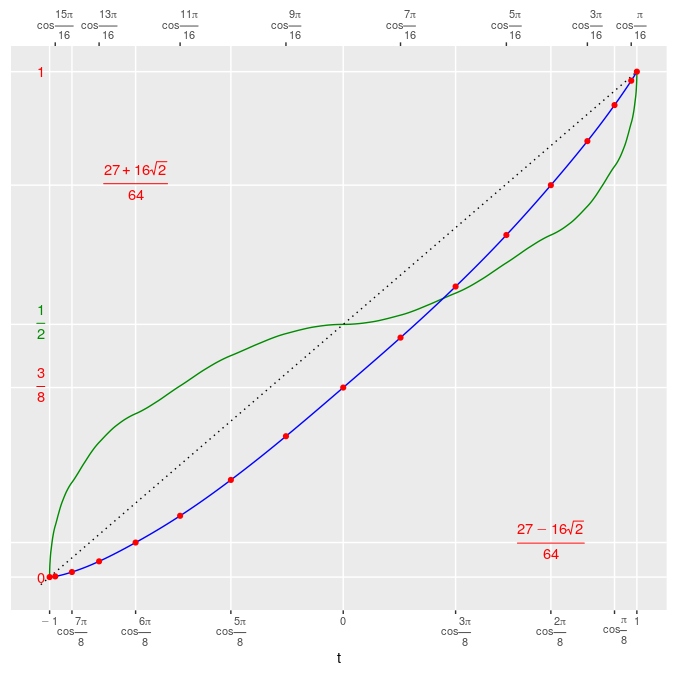
\includegraphics[width=0.95\linewidth]{core.png}
    \end{center}
    \emph{The blue line is for $\psi_{17}$, which approximates $\psi$ to double-precision. The green line is for the exact derivative of $\psi_{17}$, which approximates the derivative of $\psi$ on $\left(-1,1\right)$ in which case the latter exists. The black dotted line is for $\psi_0$. The red points are discussed in Chapter \ref{ch:Injectivity} and are the value of $\psi$ at Chebyshev-Lobatto nodes when $t = -\cos\frac{j\pi}{16}$ and $j$ is an integer between $0$ and $16$.}
\end{figure}

Both $\psi_{17}$ (in blue) and its derivative (in green) are shown in Figure \ref{fig:core}. $\psi_{17}$ is clearly an increasing function from $\mathbb{T}$ to $\mathbb{I}$, as is its derivative. It appears that a small perturbation to $\psi$ would violate one or more of our three requirements for a core function in the KSR: increasing over $\mathbb{T}$, not continuously differentiable over $\mathbb{T}$, and having a bounded derivative wherever it exists on $\mathbb{T}$. There may well be other ways to define a core function that has these three properties, but no one has. Moreover, it seems difficult to construct one that converges more rapidly than $\psi_k$ does. 

This section merely proves what is already apparent from Figure \ref{fig:core}. Since $\psi_k$ converges uniformly to $\psi$ over $\mathbb{T}$ per Lemma \ref{lem:limit}, $\psi$ inherits most of the properties of $\psi_k$ as $k \uparrow \infty$.
\begin{lemma}
  \label{lem:convexity}
  \uses{def:core}
  $\psi$ is a convex function over $\mathbb{T}$.
\end{lemma}
  
\begin{proof}
  \uses{lem:TT_recursion}
  $\psi_k\left(t\right) = \threesevenths + \offset + \frac{t}{2} + \frac{1}{2} \sum\limits_{m = 1}^k  \frac{2 T_{2^{m - 1}}\left(t\right)^2 - 1}{8^m} = \threesevenths + \offset + \frac{t}{2} + \sum\limits_{m = 1}^k  8^{-m} T_{2^{m - 1}}\left(t\right)^2 - \frac{1 - 8^{-k}}{14}$ by Lemma \ref{lem:TT_recursion}. Thus, $\psi_k$ is a weighted sum of squares plus a line, both of which are convex functions, as is their sum. The uniform limit of convex functions is a convex function, so $\psi$ is a convex function.
\end{proof}

Since $T_{2^m}$ and $\psi_k$ are polynomials, their derivatives are also polynomials.
\begin{definition}[Chebyshev polynomial of the second kind]
  \label{def:U}
  \leanok
  The second-kind Chebyshev polynomial in $r$ with index $j \geq -1$ is defined recursively as
  \begin{align*}
U_j\left(r\right) \equiv 
\begin{cases}
0 & \text{if } j = -1 \\
1 & \text{if } j = 0 \\
2r & \text{if } j = 1 \\
2 r U_{j - 1}\left(r\right) - U_{j - 2}\left(r\right) & \text{if } j > 1
\end{cases}
  \end{align*}
\end{definition}

\begin{lemma}[]
  \label{lem:T_derivative}
  \uses{def:U}
  \leanok
  If $j \geq 0$, then $\dot{T}_j\left(r\right) = j U_{j - 1}\left(r\right)$.
\end{lemma}
\begin{proof}
  \leanok
  This is already proven by induction in Mathlib. TODO: Add a succinct explanation.
\end{proof}

\begin{lemma}
  \label{lem:U_composition}
  \uses{def:U, def:T}
  $U_{-1 + 2^m}\left(t\right) = 2 \TT{m - 1}{t} U_{-1 + 2^{m - 1}}\left(t\right)$
\end{lemma}
\begin{proof}
  Differentiating both sides of the equation from Lemma \ref{lem:TT_recursion}, $\TT{m}{t} = 2\TT{m - 1}{t}^2 - 1$, and applying Lemma \ref{lem:T_derivative} implies $2^m U_{-1 + 2^m}\left(t\right) = 2^2\TT{m - 1}{t} 2^{m - 1} U_{-1 + 2^{m - 1}}\left(t\right)$, so dividing both sides by $2^m$ yields the result.
\end{proof}
Lemma \ref{lem:U_composition} allows $\dotpsi{k}{t}$ to be built up term-by-term in the same unrolled loop that evaluates $\TT{m - 1}{t}$, which only doubles its already low computational cost.
\begin{lemma}
  \label{lem:psi_k_derivative}
  \uses{def:T, def:approx, def:U}
  $\dotpsi{k}{t} = \frac{1}{2} \sum\limits_{m = 0}^k 4^{-m} U_{-1 + 2^m}\left(t\right) = \frac{1}{2} + \sum\limits_{m = 1}^k \TT{m - 1}{t} U_{-1 + 2^{m - 1}}\left(t\right)$.
\end{lemma}
\begin{proof}
  Since $\threesevenths + \offset$ is not a function of $t$, applying Lemma \ref{lem:T_derivative} to each remaining term in Definition \ref{def:approx} yields the first form and substituting for $U_{-1 + 2^m}\left(t\right)$ using Lemma \ref{lem:U_composition} yields the second form.
\end{proof}

\begin{lemma}[]
  \label{lem:positive_derivative}
  \uses{lem:psi_k_derivative}
   $\dotpsi{k}{t} \geq 2^{-k - 1} = \dot{\psi}_k\left(-1\right)$.
\end{lemma}
\begin{proof}
  It is already proven by induction in Mathlib (TODO: Add a succinct explanation) that $U_j\left(-1\right) = \left(-1\right)^j \left(j + 1\right)$. Using the first form in Lemma \ref{lem:psi_k_derivative}, $\dot{\psi}_k\left(-1\right) = \frac{1}{2} - \frac{1}{2} \sum\limits_{m = 1}^k 4^{-m} 2^m = \frac{1}{2} - \frac{1}{2} \sum\limits_{m = 1}^k 2^{-m} = 2^{-k - 1}$ by Lemma \ref{lem:geometric} with $b = 2$. Per Lemma \ref{lem:convexity}, $\psi_k$ is convex, so its derivative is an increasing function over $\mathbb{T}$ from a minimum of $2^{-k - 1}$.
\end{proof}

\begin{lemma}
  \label{lem:increasing}
  \uses{def:core}
  $\psi$ is an increasing function over $\mathbb{T}$.
\end{lemma}

\begin{proof}
  \uses{lem:positive_derivative, lem:limit}
  Lemma \ref{lem:positive_derivative} implies that $\psi_k$ is an increasing function over $\mathbb{T}$. The uniform limit of increasing functions is an increasing function, so $\psi$ is an increasing function.
\end{proof}

\begin{lemma}
  \label{lem:derivative_bound}
  \uses{lem:psi_k_derivative}
  $\dotpsi{k}{t} \leq 1 - 2^{-k - 1} = \dot{\psi}_k\left(1\right)$
\end{lemma}

\begin{proof}
  It is already proven by induction in Mathlib (TODO: Add a succinct explanation) that $U_j\left(1\right) = j + 1$. Using the first form in Lemma \ref{lem:psi_k_derivative}, $\dot{\psi}_k\left(1\right) = \frac{1}{2} + \frac{1}{2} \sum\limits_{m = 1}^k 2^{-m} = 1 - 2^{-k - 1}$ by Lemma \ref{lem:geometric} with $b = 2$. Per Lemma \ref{lem:convexity}, $\psi_k$ is convex, so its first derivative is an increasing function over $\mathbb{T}$ to a maximum of $1 - 2^{-k - 1}$.
\end{proof}

\begin{lemma}
  \label{lem:contraction}
  \uses{def:core}
  $\psi$ is a weak contraction over $\mathbb{T}$.
\end{lemma}

\begin{proof}
  \uses{lem:derivative_bound, lem:limit}
  Lemma \ref{lem:derivative_bound} implies $\psi_k$ is Lipschitz continuous with a constant of $1 - 2^{-k - 1}$. The uniform limit of Lipschitz continuous functions is Lipschitz continuous. Although the derivative of $\psi$ does not exist at $t = 1$, the supremum of the derivative of $\psi$ is $1$, making it a weak contraction.
\end{proof}

\begin{lemma}
  \label{lem:codomain}
  \uses{def:approx, def:core}
  The codomain of $\psi_k$ is $\mathbb{I}$, as is the codomain of $\psi$.
\end{lemma}

\begin{proof}
  \uses{lem:convexity, lem:fixed_points, lem:geometric, lem:TT_recursion}
  Lemma \ref{lem:convexity} implies $\psi_k$ and $\psi$ are increasing functions over $\mathbb{T}$, which are minimized at $t = -1$ and maximized at $t = 1$.
  \begin{itemize}
      \item If $t = 1$, Lemma \ref{lem:fixed_points} implies $\TT{m}{1} = 1$. Thus, $\psi_k\left(1\right) = \threesevenths + \offset + \frac{1}{2} + \frac{1}{2} \sum\limits_{m = 1}^k 8^{-m} = \threesevenths + \offset + \frac{1}{2} + \frac{1}{2} \frac{1 - 8^{-k}}{7} = 1$ by Lemma \ref{lem:geometric} with $b = 8$. Similarly, $\psi\left(1\right) = \threesevenths + \frac{1}{2} \sum\limits_{m = 0}^\infty 8^{-m} = \threesevenths + \frac{1}{2} \frac{8}{7} = 1$.
      \item If $t = -1$, $\TT{1}{-1} = 2 \TT{0}{-1}^2 -1 = 1$ by Lemma \ref{lem:TT_recursion} and Lemma \ref{lem:fixed_points} implies $\TT{m}{-1} = 1$ as well for all $m > 1$.  Thus, $\psi_k\left(-1\right) = 0 = \psi\left(-1\right)$ by the same reasoning as in the $t = 1$ case, except the contribution when $m = 0$ is $-\frac{1}{2}$ rather than $\frac{1}{2}$.
  \end{itemize}
\end{proof}
\noindent Hence, the unusual constant, $\offset$, in the definition of $\psi_k$ anchors its codomain to $\mathbb{I}$ for all $k$.

\section{Differentiability}\label{sec:Differentiability}

The fact that $\psi_k$ converges uniformly to $\psi$ per Lemma \ref{lem:limit} does not imply that $\dot{\psi}_k$ converges in any sense to $\dot{\psi}$, in part because the derivative of $\psi$ does not even exist at $-1$ and $1$. However, the derivative of $\psi$ can be shown to exist on $\left(-1,1\right)$ and $\dot{\psi}_k$ converges to it as $k \uparrow \infty$. 

\begin{proposition}
  \label{prop:derivative}
  \uses{def:core}
  If $t \in \left(-1,1\right)$, $\dot{\psi}\left(t\right)$ exists.
\end{proposition}
\begin{proof}
  \uses{lem:TT_recursion, lem:increasing}
  We start with the definition of a derivative,
  \begin{eqnarray*}
    \dot{\psi}\left(t\right) = \lim\limits_{h \rightarrow 0} \frac{\psi\left(t + h\right) - \psi\left(t\right)}{h} = 
    \lim\limits_{h \rightarrow 0} \frac{\frac{1}{2} \sum\limits_{m = 0}^\infty 8^{-m} \left(\TT{m}{t + h} - \TT{m}{t}\right)}{h}.
  \end{eqnarray*}
  Pulling the $\TT{0}{t + h} - \TT{0}{t} = t + h - t = h$ term out of the sum, applying the recursion from Lemma \ref{lem:TT_recursion}, simplifying, and factoring a difference of squares implies
  \begin{eqnarray*}
    \dot{\psi}\left(t\right) &=& \frac{1}{2} + \lim\limits_{h \rightarrow 0} \frac{\frac{1}{2}\sum\limits_{m = 1}^\infty 8^{-m} \left(2\TT{m - 1}{t + h}^2 - 1 - \left(2\TT{m - 1}{t}^2 - 1\right)\right)}{h} \\  
    &=& \frac{1}{2} + \lim\limits_{h \rightarrow 0} \frac{\frac{1}{2}\sum\limits_{m = 1}^\infty 8^{-m} 2\left(\TT{m - 1}{t + h}^2 - \TT{m - 1}{t}^2\right)}{h} \\
    &=& \frac{1}{2} + \lim\limits_{h \rightarrow 0} \frac{\frac{1}{2}\sum\limits_{m = 1}^\infty 8^{-m} 2\left(\TT{m - 1}{t + h} + \TT{m - 1}{t}\right) \left(\TT{m - 1}{t + h} - \TT{m - 1}{t}\right)}{h}.
  \end{eqnarray*}
  Repeatedly applying the recursion from Lemma \ref{lem:TT_recursion} to the difference term, simplifying, and factoring a difference of squares in the same way implies
  \begin{eqnarray*}
    \dot{\psi}\left(t\right) &=& \frac{1}{2} + \lim\limits_{h \rightarrow 0} \frac{\frac{1}{2} \sum\limits_{m = 1}^\infty 8^{-m} 2^{m}\left[\prod\limits_{j = m - 1}^0 \left(\TT{j}{t + h} + \TT{j}{t}\right)\right]\left(\TT{0}{t + h} - \TT{0}{t}\right)}{h} \\  
    &=& .\frac{1}{2} + \lim\limits_{h \rightarrow 0} \frac{1}{2} \sum\limits_{m = 1}^\infty 4^{-m} \prod\limits_{j = m - 1}^0 \left(\TT{j}{t + h} + \TT{j}{t}\right),
  \end{eqnarray*}
  where the last line again follows from the fact that $\TT{0}{t + h} - \TT{0}{t} = t + h - t = h$. Since $h$ has been cleared from the denominator and $\psi$ is increasing per Lemma \ref{lem:increasing}, we can apply the Weierstrass M-test again, after noting that the absolute value of $2^{-m}$ multiplied by a product of numbers on $\left(-1,1\right)$ is bounded by $2^{-m}$,
  \begin{eqnarray*}
    \dot{\psi}\left(t\right)
    &=& \frac{1}{2} + \frac{1}{2} \sum\limits_{m = 1}^\infty 4^{-m} 2^m \prod\limits_{j = m - 1}^0 \TT{j}{t}
    \leq \frac{1}{2} + \frac{1}{2} \sum\limits_{m = 1}^\infty 2^m = \frac{1}{2} + \frac{1}{2} = 1.
  \end{eqnarray*}
  Thus, $\dot{\psi}$ is well-defined on $\left(-1,1\right)$.
\end{proof}

If $0 < q < 2n$ and $\psi_{p,q}\left(t\right) \propto \psi\left(x_p - \frac{q}{2n}\right)$, then this inner function is continuously differentiable because neither $-1$ nor $1$ is a feasible point.

\begin{lemma}[]
  \label{lem:derivative_convergence}
  \uses{lem:psi_k_derivative}
  $\dot{\psi}_k$ converges uniformly to $\dot{\psi}$ on $\left(-1,1\right)$.
\end{lemma}
\begin{proof}
  \uses{lem:derivative_bound}
  Lemma \ref{lem:derivative_bound} implies the sequence of functions $\dot{\psi}_k$ is bounded by the sequence $1 - 2^{-k - 1} = \dot{\psi}_k\left(1\right)$, so $\dot{\psi}_k$ converges uniformly to $\dot{\psi}$ on $\left(-1,1\right)$.
\end{proof}

\begin{lemma}
  \label{lem:ODE}
  \uses{def:T, def:U}
  If $t^2 \neq 1$, then $\ddot{T}_{2^m}\left(r\right) = \frac{t}{1 - t^2} \dot{T}_{2^m}\left(t\right) - \frac{4^m}{1 - t^2} \TT{m}{t}$.
\end{lemma}
\begin{proof}
  \uses{lem:TT_recursion}
  If $m = 0$, then $\TT{0}{t} = t$ and per Lemma \ref{lem:TT_recursion}, if $m > 0$, $\TT{m}{t} = 2\TT{m - 1}{t}^2 - 1$. Thus, $\TT{m}{t}$ is a polynomial where all exponents are even numbers except for the linear term. If we differentiate $\TT{m}{t}$, the coefficients are multiplied by the exponents and the exponents are decremented, which causes the linear term to become a constant. If we differentiate again, the coefficients are multiplied by the new exponents and the exponents are decremented again. If we multiply the second derivative by $1 - t^2$, the result is equal to $t \dot{T}_{2^m}\left(t\right) - \left(2^m\right)^2 \TT{m}{t}$., Thus if $t^2 \neq 1$, we can divide both sides by $1 - t^2$, which yields the result.
\end{proof}

\begin{lemma}
  \label{lem:second_derivative}
  \uses{def:approx, lem:psi_k_derivative}
  If $t \in \mathbb{T}$, then $\ddotpsi{k}{t} = \frac{t}{1 - t^2} \dotpsi{k}{t} - \frac{1}{1 - t^2} \sum\limits_{m = 0}^k 2^{-m} \TT{m}{t}$, and $\ddot{\psi}_k$ converges uniformly to $\ddot{\psi}$ on $\left(-1,1\right)$.
\end{lemma}
\begin{proof}
  \uses{lem:ODE, lem:derivative_convergence, lem:geometric}
  After differentiating Definition \ref{def:approx} twice, applying Lemma \ref{lem:ODE} to each term in the sum, canceling common factors, we obtain the above expression for $\ddotpsi{k}{t}$. Since $\dot{\psi}_k$ converges uniformly by Lemma \ref{lem:derivative_convergence}, $\TT{m}{t} \in \mathbb{T}$, and $\sum\limits_{m = 0}^\infty \left|2^{-m} \TT{m}{t}\right| \leq \sum\limits_{m = 0}^\infty 2^{-m} = 2$ by Lemma \ref{lem:geometric} with $b = 2$, $\ddot{\psi}_k$ converges uniformly.
 \end{proof}
\noindent Thus, $\ddotpsi{k}{t}$ can be computed within the same unrolled loop that calculates $\TT{m}{t}$ and $U_{-1 + 2^m}\left(t\right)$ at the cost of just an additional accumulation of the second term in $\ddotpsi{k}{t}$. However, it seems \underline{unlikely} that $\psi$ has a third derivative on $\left(-1,1\right)$ because differentiating under the sum again would cause the sum to diverge.

\chapter{Injectivity}\label{ch:Injectivity}
It must also be shown that $\Psi_q$ is an injective function when used with our candidate for a core function. To do so, it is better in this chapter to utilize the trigonometric representation of $T_{2^k}$.
\begin{definition}[Normalizer]
  \label{def:Lambda}
  $\Lambda \equiv \sum\limits_{p = 1}^n \lambda^{p - 1}$ where $\lambda > 0$.
\end{definition}
\begin{definition}[Scale factor]
  \label{def:lambda_p}
  \uses{def:Lambda}
  $\lambda_p \equiv \frac{\lambda^{p - 1}}{\Lambda}$.
\end{definition}
\begin{definition}[Basic family]
  \label{def:Psi}
  \uses{def:lambda_p}
  $\Psi_q\left(x_1, x_2, \dots, x_n\right) \equiv \sum\limits_{p = 1}^n \lambda_p \psi\left(x_p - \frac{q}{2n}\right)$.
\end{definition}
\noindent These definitions are convenient and do not alter Sprecher's conclusion that the KSR can hold with a weakly contractive core function because the outer functions could simply multiply $\Psi_q$ by $\Lambda$ to obtain Sprecher's form again.
\begin{lemma}
  \label{lem:Psi_q_codomain}
  \uses{def:Psi}
  The codomain of $\Psi_q$ is $\mathbb{I}$.
\end{lemma}
\begin{proof}
  \uses{lem:codomain}
  Per Lemma \ref{lem:codomain}, the codomain of $\psi$ is $\mathbb{I}$. Since $0 < \lambda_p \leq \frac{1}{\Lambda}$ and $\sum\limits_{p = 1}^n \lambda_p = 1$, the result follows.
\end{proof}

\begin{lemma}[]
  \label{lem:trigonometric}
  \uses{def:T}
  \leanok
  If $t \in \mathbb{T}$, then $T_j\left(t\right) = \cos\left(j \cos^{-1}t\right)$.
\end{lemma}
  
\begin{proof}
  \leanok
  Let $t = \cos \theta$. If $j = 0$, then $T_0\left(t\right) = 1 = \cos\left(0 \theta\right)$. If $j = 1$, then $T_1\left(t\right) = t = \cos\left(1 \theta\right)$. It remains to show for $j > 1$ that the recursion in Definition \ref{def:T} is satisfied: $T_j\left(t\right) = 2 \cos \theta \cos\left(\left(j - 1\right) \theta\right) - \cos\left(\left(j - 2\right) \theta\right)$. The first term can be rewritten as $2\cos \theta \cos\left(\left(j - 1\right) \theta\right) = \cos\left(\theta - \left(j - 1\right)\theta\right) + \cos\left(\theta + \left(j - 1\right)\theta\right) = \cos\left(\left(j - 2\right)\theta\right) + \cos\left(j \theta\right)$, so $T_j\left(t\right) = \cos\left(j \theta\right)$.
\end{proof}

\begin{lemma}[Chebyshev-Lobatto nodes]
  \label{lem:nodes}
  The $1 + 2^k$ extrema of $T_{2^k}$ are called (Chebyshev-Lobatto) nodes and occur at $\tau \equiv -\cos\frac{j\pi}{2^k}$ for each natural number $j \leq 2^k$.
\end{lemma}
\begin{proof}
  \uses{lem:trigonometric}
  If $\tau \equiv -\cos\frac{j\pi}{2^k}$, then $\TT{k}{\tau} = \cos\left(2^k \cos^{-1}\left(\cos \frac{-j\pi}{2^k}\right)\right) = \cos\left(-j\pi\right)$. If $j$ is even, $\TT{k}{\tau} = 1$ and if $j$ is odd $\TT{k}{\tau} = -1$.
\end{proof}
The approximation literature also defines nodes when the index of the Chebyshev polynomial is not a power of two, but that case is not applicable to us. Our nodes are also constructible numbers.
\begin{definition}[Real constructible number field, $\mathbb{F}$]
  \label{def:F}
  A real number is constructible if and only if it can be computed using only integers and a finite number of additions, subtractions, multiplications, (real) divisions, and square roots (of non-negative numbers). Such numbers form a field, $\mathbb{F}$.
\end{definition}
\begin{lemma}
  \label{lem:constructible}
  \uses{def:F}
  If $0 \leq j \leq 2^k$, then $-\cos\frac{j\pi}{2^k} \in \mathbb{F}$.
\end{lemma}
\begin{proof}
   If $j = 0$, then $\cos 0 = 1$ and if $j = 2^k$, then $\cos \pi = -1$, which are both constructible numbers and serve as base cases. If $k > 0$, utilize the fact that $\cos\frac{\vartheta}{2} = \left(-1\right)^{\left\lfloor \frac{\vartheta + \pi}{2\pi} \right\rfloor} \sqrt{\frac{1 + \cos \vartheta}{2}}$ repeatedly until reaching one of the two base cases after $k$ iterations; the result is a constructible number. Multiplying a constructible number by $-1$ yields a constructible number.
\end{proof}

\begin{lemma}
  \label{lem:psi_k_constructible}
  \uses{def:F}
  If $0 \leq j \leq 2^k$, $\psi_{k}\left(-\cos\frac{j\pi}{2^k}\right) \in \mathbb{F}$.
\end{lemma}
\begin{proof}
   \uses{lem:constructible, lem:TT_recursion, def:approx}
   If $m = 0$, then $\TT{0}{-\cos\frac{j\pi}{2^k}} = -\cos\frac{j\pi}{2^k} \in \mathbb{F}$ by Lemma \ref{lem:constructible}. Per Lemma \ref{lem:TT_recursion}, by induction on $m$, $\TT{m}{-\cos\frac{j\pi}{2^k}} = 2 \TT{m - 1}{-\cos\frac{j\pi}{2^k}}^2 - 1 \in \mathbb{F}$ because it only involves arithmetic operations on constructible numbers. By Definition \ref{def:approx}, $\psi_k\left(-\cos\frac{j\pi}{2^k}\right) = \threesevenths + \offset + \halfsum{0}{k}{-\cos\frac{j\pi}{2^k}} \in \mathbb{F}$ because it only involves arithmetic operations on constructible numbers.
\end{proof}


The red points in Figure \ref{fig:core} are the values of $\psi$ at these nodes when $k = 4$, which crucially can be calculated \emph{exactly} in a finite number of steps from $\psi_4$ or better, so they too are constructible.

\begin{lemma}[Magic trick]
  \label{lem:magic}
  \uses{def:approx, def:core}
  If and only if $0 \leq j \leq 2^k$, $\psi_k\left(-\cos\frac{j\pi}{2^k}\right) = \psi\left(-\cos\frac{j\pi}{2^k}\right)$.
\end{lemma}
\begin{proof}
  \uses{lem:fixed_points, lem:geometric}
  If $\tau = -\cos\frac{j\pi}{2^k}$, then Lemma \ref{lem:fixed_points} implies $\TT{k + 1}{\tau} = 1$ is a fixed point. By Lemma \ref{lem:geometric} with $b = 8$, $\psi\left(\tau\right) = \threesevenths + \halfsum{0}{k}{\tau} + \frac{1}{2}\sum\limits_{m = k + 1}^\infty 8^{-m} = \threesevenths + \halfsum{0}{k}{\tau} + \offset = \psi_k\left(\tau\right)$. Conversely, if $\TT{k}{t} = \frac{1}{2}$, then Lemma \ref{lem:fixed_points} implies $\TT{k + 1}{t} = -\frac{1}{2}$ is the other fixed point. Although Lemma \ref{lem:geometric} implies $\psi\left(t\right) = \threesevenths + \halfsum{0}{k}{t} - \frac{1}{4}\sum\limits_{m = k + 1}^\infty 8^{-m} = \threesevenths + \halfsum{0}{k}{t} - \frac{8^{-k}}{28}$ can be computed in a finite number of arithmetic operations and thus is constructible, the result is not equal to $\psi_k\left(t\right)$. Otherwise $\psi\left(t\right)$ cannot be computed in any finite number of operations.
\end{proof}
\noindent If $\tau \equiv -\cos \frac{1\pi}{2^1} = 0$, Lemma \ref{lem:magic} implies $\psi_1\left(0\right) = \frac{3}{8} = \psi\left(0\right)$. If $\tau \equiv -\cos\frac{\left(2 \mp 1\right)\pi}{2^2} = \frac{\mp 1}{\sqrt{2}}$, Lemma \ref{lem:magic} implies $\psi_2\left(\frac{\mp 1}{\sqrt{2}}\right) = \frac{27 \mp 16 \sqrt{2}}{64} = \psi\left(\frac{\mp 1}{\sqrt{2}}\right)$ can be calculated in a finite number of steps, neither is rational but both are constructible. These three points are highlighted in Figure \ref{fig:core}. Values of $\psi\left(t\right)$ when $t \approx \tau$ are near $\psi\left(\tau\right)$ since $\psi$ is a weak contraction but, in principle, require evaluating an infinite sum. In practice, it is only necessary to evaluate $\psi_{17}\left(t\right)$ to obtain accurate results.

Although $\psi_k$ is defined on $\mathbb{T}$, in this chapter we will take $\psi_k$ to be a function of nodes, which can be extended to function over $\mathbb{T}$. The KST literature usually defines an inner function to be rational on rational numbers, and then extends the inner function to irrational numbers by connecting it with horizontal segments. Our approach can be seen as a slight variation on the historical one.
\begin{lemma}
  \label{lem:extension}
  \uses{def:approx, def:core}
  If $0 < j < 2^k$ and $j \neq 2^{k - 1}$ and $\tau \equiv -\cos\frac{j\pi}{2^k}$, then $\TT{m}{\tau}$, $\psi_k\left(\tau\right)$, and $\psi\left(\tau\right)$ can all be considered to be in the extension field $\mathbb{Q}\left(\tau\right)$.
\end{lemma}
\begin{proof}
  If $j = 0$, $j = 2^{k - 1}$, or $j = 2^k$, then $-\cos\frac{j\pi}{2^k}$ is $-1$, $0$, or $1$ respectively, which are integers. In those cases, $\TT{m}{-\cos\frac{j\pi}{2^k}} \in \mathbb{Z}$, $\psi_k\left(-\cos\frac{j\pi}{2^k}\right) \in \mathbb{Q}$, and $\psi\left(-\cos\frac{j\pi}{2^k}\right) \in \mathbb{Q}$, so there is no extension of the rational number field. If $\tau \equiv -\cos\frac{j\pi}{2^k} \notin \mathbb{Z}$, these three functions thereof are in $\mathbb{Q}\left(\tau\right)$.
\end{proof}

\begin{lemma}
  \label{lem:injective}
  \uses{def:F, def:Psi}
  If $\lambda > 0$ is algebraic or transcendental, then $\Psi_q$ is an injective function on nodes.
\end{lemma}
\begin{proof}
  \uses{lem:magic}
  For some sufficiently large $k$, assume $x_p - \frac{q}{2n}$ is some node for each $p$ (not necessarily the same node) and similarly assume $x_p^\prime - \frac{q}{2n}$ is also some node for each $p$. If $\Psi_q\left(x_1, x_2, \dots, x_n\right) = \Psi_q\left(x_1^\prime, x_2^\prime, \dots, x_n^\prime\right)$, then we can apply Definition \ref{def:Psi} to rearrange this condition as
  \begin{eqnarray*}
      \frac{\psi\left(x_1 - \frac{q}{2n}\right) - \psi\left(x_1^\prime - \frac{q}{2n}\right)}{\Lambda} &=& \frac{\sum\limits_{p = 2}^n\lambda^{p - 1} \left(\psi\left(x_p^\prime - \frac{q}{2n}\right) - \psi\left(x_p - \frac{q}{2n}\right)\right)}{\Lambda}, \\
      \psi_k\left(x_1 - \frac{q}{2n}\right) - \psi_k\left(x_1^\prime - \frac{q}{2n}\right) &=& \sum\limits_{p = 2}^n\lambda^{p - 1} \left(\psi_k\left(x_p^\prime - \frac{q}{2n}\right) - \psi_k\left(x_p - \frac{q}{2n}\right)\right),
  \end{eqnarray*}
  where Lemma \ref{lem:magic} allows us to substitute $\psi_k$ for $\psi$ in the second line. Its right-hand side is zero if $x_p = x_p^\prime$ for all $p \geq 2$ or else it is a number in the same field as $\lambda$. The left-hand side is a constructible number as it is the difference between two constructible numbers. If $\lambda$ is an algebraic or transcendental number, then the two sides cannot be equal unless $x_p = x_p^\prime$ for all $p$. Thus, $\Psi_q\left(x_1, x_2, \dots, x_n\right) = \Psi_q\left(x_1^\prime, x_2^\prime, \dots, x_n^\prime\right) \implies x_p = x_p^\prime \forall p$, which defines an injective function.
\end{proof}

\begin{proposition}
  \label{prop:injective}
  \uses{def:Psi}
  If $\lambda > 0$ is algebraic or transcendental, then $\Psi_q$ is an injective function on $\mathbb{I}^n$.
\end{proposition}
\begin{proof}
  \uses{lem:injective}
  Nodes are dense in $\mathbb{T}$ with a Probability Density Function of $\frac{1}{\pi \sqrt{1 - \tau^2}} > 0$ as $k \uparrow \infty$. Thus, Lemma \ref{lem:injective} implies $\Psi_q$ is also injective on $\mathbb{I}^n$.
\end{proof}

Sprecher and others use essentially the same trick with an irrational value of $\lambda$ that elevates non-zero rational values to the real number field. A node is already irrational unless it is among the integers $-1$, $0$, or $1$, so $\psi\left(\tau\right)$ is irrational unless it is among $\psi\left(-1\right) = 0$, $\psi\left(0\right) = \frac{3}{8}$, or $\psi\left(1\right) = 1$. However, $\tau$ and $\psi\left(\tau\right) = \psi_k\left(\tau\right)$ are always constructible numbers that generally extend the rational number field per Lemma \ref{lem:extension}. We simply extend again with an algebraic or transcendental $\lambda > 0$.

\chapter{Outer Functions}\label{ch:OuterFunctions}

The number of distinct outer functions can also be reduced to one by shifting the argument.
\begin{definition}
  \label{def:outer}
  $\chi_q\left(\Psi_q\left(x_1, x_2, \dots, x_n\right)\right) \equiv \chi\left(\Psi_q\left(x_1, x_2, \dots, x_n\right) + q\right)$.
\end{definition}

Kahane's geometric interpretation of the KST goes like this. Let $\Gamma_p$ denote an ``increasing curve'' in $\mathbb{R}^{2n + 1}$ for the equation $X_q\left(x\right) = \lambda_p \psi\left(x - \frac{q}{2n}\right)$. Let $E \equiv \lambda_1 \Gamma + \lambda_2 \Gamma + \dots + \lambda_n \Gamma$, so $E \subset \mathbb{I}^{2n + 1}$. Then,
\begin{enumerate}
  \item The mapping $\Gamma_1 \times \Gamma_2 \times \dots \times \Gamma_n$ is injective so $E$ is a distorted cube
  \item $E$ is an interpolation set in the sense that every continuous function on can be written in the form $\chi_1\left(X_1\right) + \chi_2\left(X_2\right) + \dots + \chi_{2n}\left(X_{2n}\right)$.
\end{enumerate}

\begin{definition}[Helson set]
  \label{def:Helson_set}
``[A] Helson set in a locally compact abelian group $G$ is a closed set $E$ such that the algebra $A(E)$ of restrictions to $E$ of functions in $A(G)$ (Fourier transforms of summable functions on the dual group) coincides with $C(E)$, the algebra of all continuous functions on $E$." (translated from page 91 of Kahane 1978) where 
\end{definition}

\begin{lemma}
  \label{lem:not_Helson}
  \uses{def:Helson_set}
  ``If $E$ contains the algebraic sum of two infinite sets, $E$ is not a Helson set.''
\end{lemma}
\begin{proof}
  See page 91 of Kahane 1978; it has to do with violating a mesh condition.
\end{proof}

\begin{lemma}
  \label{lem:polynomial}
  \uses{def:Helson_set}
  If $\gamma$ coincides on any subinterval of $\mathbb{I}$ with a polynomial of degree less than $n$, then $\{\gamma\left(\Psi_1\right), \gamma\left(\Psi_2\right), \dots, \gamma\left(\Psi_{2n}\right)\}$ is not a Helson set.
\end{lemma}
\begin{proof}
  Also has do to with the mesh condition.
\end{proof}

\begin{proposition}
  \label{prop:Helson}
  \uses{def:Helson_set}
  If $\gamma$ is an increasing homeomorphism of $\mathbb{I}$ that does not coincide with a polynomial of degree less than $n$ on any subinterval of $\mathbb{I}$, then $\gamma\left(E\right)$ is quasi-surely a Helson set. Moreover, the condition on $\gamma$ is necessary and sufficient, and $\chi_q \in A^+\left(\mathbb{I}\right)$ where $A^+\left(\mathbb{I}\right)$ is a class of functions $\chi\left(z\right) = \sum\limits_{j = 0}^\infty \widehat{a}_j e^{2\pi \imath j z}$.
\end{proposition}
\begin{proof}
   ``The proof relies on the following proposition, which is very similar to one given in [Kahane's 1975 article] p. 233 and can be proven in the same way.'' 
   \begin{quote}
    Let $B\left(\mathbb{I}\right)$ be a Banach space contained in $C\left(\mathbb{I}\right)$ and satisfying hypothesis (H): there exists $c > 0$ such that, for any $\delta > 0$, there exist finite sets $D_p\subset I$ (for $p = 1, 2, \ldots, n$) with at least one point in every subinterval of length $\delta$, such that the mapping $D_1\times D_2\times \dots \times D_n \to D_1 + D_2 + \ldots + D_n$ is injective, and for any function $u$ of modulus 1 on the set $D_1 + D_2 + \ldots + D_n$, there exists $\chi\in B\left(\mathbb{I}\right)$, with $\left|\left|\chi\right|\right|_{B\left(\mathbb{I}\right)} \leq c$ and $\left|\left|\chi\right|\right|_{C\left(\mathbb{I}\right)} = 1$, where $\chi = u$ on $D_1 + D_2 + \ldots + D_n$. Then one can choose $\chi \in B\left(\mathbb{I}\right)$.
    \end{quote}
    [I]t follows [from Kronecker's theorem] that any function of modulus 1 on $\mathbb{I}$ can be written as $\sum\limits_{j = 1}^\infty a_j e^{\imath j z}$, with $\sum\limits_{j = 1}^\infty \left|a_j\right| \leq 2$. By applying the proposition, we can therefore take $\chi \in (A \circ \gamma)\left(\mathbb{I}\right)$ as soon as homeomorphism $\gamma$ satisfies the condition:
    \begin{quote}
    For every $\delta > 0$, there exist finite sets $D_p \subset \mathbb{I}$ (for $p = 1, 2, \ldots, n$) at least one point in every subinterval of $\mathbb{I}$ of length $\delta$, such that the mapping $D_1 \times D_2\times \ldots D_n \to D_1 + D_2 + \ldots + D_n$ is injective, and $\gamma(D_1 + D_2 + \ldots + D_n)$ is a rationally independent set.
   \end{quote}
\end{proof}

Then $\chi_q\left(\gamma\left(\Psi_q\left(x_1, x_2, \dots, x_n\right)\right)\right) = \sum\limits_{j = 0}^\infty \widehat{a}_j e^{2\pi \imath j \left(\gamma\left(\Psi_q\left(x_1, x_2, \dots, x_n\right)\right) + q\right)} = \sum\limits_{j = 0}^\infty \widehat{a}_j e^{2\pi \imath j \left(\gamma\left(\Psi_q\left(x_1, x_2, \dots, x_n\right)\right)\right)}$ because it is periodic. In practice, we would have to estimate a (truncated) sequence of coefficients to calibrate to a particular target function.

\chapter*{Bibliography}

    \bibliographystyle{plain} % Choose your preferred citation style

    \bibliography{references}  % Name of your BibTeX file

    \nocite{*}  % Include all entries in the bibliography

